%-------------------------------------------------------------------------------
%-------------------------------------------------------------------------------
%-------------------------------------------------------------------------------
\chapter{Exploitation de données}
%-------------------------------------------------------------------------------
%-------------------------------------------------------------------------------
\thispagestyle{empty}
%--------------------------------------------------------------------------
%--------------------------------------------------------------------------
%--------------------------------------------------------------------------
\section{Introduction}
%--------------------------------------------------------------------------
%--------------------------------------------------------------------------
%--------------------------------------------------------------------------
Le but de ce T.P. est de d'utiliser le langage SQL pour exploiter une base de données.

Un base de données simple est une ensemble de données regroupées 
%--------------------------------------------------------------------------
\begin{itemize}
\item par ligne, ce sont les données d'un objet (ici les communes de France continentale)
\item par colonnes, ce les différents type de données (population, département, \dots)
\end{itemize}
%--------------------------------------------------------------------------

Nous allons utiliser des données fournies par l'INSEE, résultat des recensements.

Ce fichier est relativement simple mais très long : plus de 35000 lignes.

On pourrait le traiter à l'aide d'un tableur (c'est son format d'origine).

Cependant même les questions simples :
%--------------------------------------------------------------------------
\begin{itemize}
\item quelles sont les villes de plus de 200 000 habitants ?
\item quelle est la commune la plus étendue (\type{surf} en km$^2$) ?
\item quelles sont les communes dont la population a plus que doublé depuis 1968 ?
\end{itemize}
%--------------------------------------------------------------------------
demanderaient des manipulations qui seraient longues à effectuer.

Le format choisi pour ces T.P. est \type{SQL Lite} : d'autres formats sont possibles (\type{MySQL}, \type{postgreSQL}, \type{Oracle}, \dots) mais tous partagent le cœur des fonctions \type{SQL}.
%--------------------------------------------------------------------------
\subsection{sqlitebrowser}
%--------------------------------------------------------------------------
En général l'intérêt d'une base de données est qu'elle peut être utilisée dans un réseau : la mise en place est assez lourde mais le partage d'une même base par plusieurs utilisateurs est un gros avantage. Pour ce T.P. nous allons nous contenter d'un dispositif plus simple : chaque poste exploitera sa base de données avec le logiciel  \textsc{sqlitebrowser}.

Il faut commencer par copier la base de données sur le bureau (Windows) ou dans le répertoire local à votre nom (Linux). La base disponible dans le dossier de votre classe dans le disque \type{Public} : \type{communes.sqlite}.

On peut ensuite lancer le logiciel :

\[
%--------------------------------------------------------------------------
\begin{tabular}{|p{7cm}|p{7cm}|}
\hline
\bf Windows  & \bf Linux \\ 
\hline
Copier le logiciel \textsc{sqlitebrowser} depuis le disque \type{P:} du réseau vers le bureau et le lancer
&
Ouvrir \textsc{sqlitebrowser} dans le menu des application, sous-menu \type{programmation}. \\ 
\hline
\end{tabular}
%--------------------------------------------------------------------------
\]

Ouvrir la base de données \type{communes.sqlite} depuis le menu \type{Files/Fichiers}, 

item \type{Open Database/Ouvrir une base de données}.

Le logiciel présente plusieurs onglets,  nous en utiliserons 3.
%--------------------------------------------------------------------------
\begin{itemize}
\item L'onglet par défaut, \type{Database Structure/Structure de la base de données}, permet de voir l'agencement des différentes tables. Notre premier TP se contente d'une seule table.
C'est ici que l'on peut s'assurer du nom des variables.
\item L'onglet \type{Browse Data/Parcourir les données} permet de voir toutes les données comme dans un tableur : en général il n'est pas utilisable car les tables auront une grande taille.
\item L'onglet \type{Execute SQL/Exécuter le SQL} est l'endroit où nous allons travailler.

On entre la commande dans la fenêtre \type{SQL} et on la fait exécuter en cliquant sur la flêche (ou sur \type{[F5]}).
\end{itemize}
%--------------------------------------------------------------------------
\begin{center}
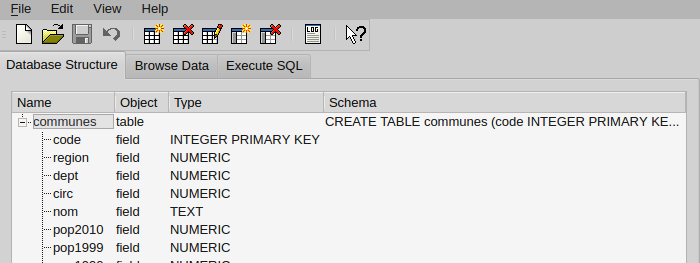
\includegraphics[scale=0.4]{Images/14_figure1}
\end{center}
%--------------------------------------------------------------------------
\subsection{sqlitebrowser}
%--------------------------------------------------------------------------
L'objectif est d'extraire des informations de la base que ces informations soient déjà présentes ou qu'elles soient extrapolables. Le langage SQL est différent de Python : en effet on demande simplement le résultat souhaité sans avoir besoin d'expliquer comment y parvenir, il le fait tout seul. On parle de {\bf langage logique}. Les questions seront appelées {\bf requêtes}.

L'ordre des instructions dans une requête est fixé :

\begin{lstlisting}[language=SQL]
SELECT ...
FROM ...
(WHERE ...)
(GROUP BY ...)
(HAVING ...)
(ORDER BY ...)
(LIMIT ...)
(OFFSET ...)
\end{lstlisting}

Seules les deux premières instructions sont obligatoires. Les instructions à partir de \type{FROM} sont exécutées dans l'ordre, \type{SELECT} chapeaute la requête.

\begin{description}
    \item[Select] est suivi de l'énumération des informations que l'on veut voir.
    \item[From] est suivi du nom de la table utilisée. Pour l'instant on se contentera d'y écrire le nom de la seule table dont on dispose : \type{from communes}. Le cours montrera l'utilité de cette instruction qui met en place l'aspect {\bf relationnel} d'une base de données.
    \item[Where] est suivi des conditions que doivent vérifier les informations que l'on veut visualiser. 
    \item[Group by] 
    \item[Having] Ces instructions seront l'objet du TP suivant
    \item[Order by] suivi d'un nom permet de trier par ordre croissant selon les valeurs de la colonne. On peut faire suivre par \type{desc} si on veut un ordre décroissant.
    \item[Limit] n'est utile qu'avec une instruction \type{Order by}. Il permet de limiter le nombre de résultats affichés
    \item[Offset] n'est utile qu'avec une instruction \type{Limit}. Il permet de décaler les instructions. \type{Limit 3 Offset 4} affiche les résultats des rangs 5 à 7.
\end{description}

%--------------------------------------------------------------------------
\newpage
%--------------------------------------------------------------------------
\section{Requêtes}
%--------------------------------------------------------------------------
%--------------------------------------------------------------------------
\subsection{SELECT}
%--------------------------------------------------------------------------
Dans cette partie, on illustre quelques possibilités de choix de colonnes mais, pour ne pas obtenir des résultats trop longs, on pourra ajouter une instruction de filtrage, par exemple,
%--------------------------------------------------------------------------
\begin{lstlisting}[language=SQL]
select 
from 
where nom = "Sainte Colombe"
\end{lstlisting}
%--------------------------------------------------------------------------
Comme le nom d'une ville est une chaîne de caractères, il faut l'encadrer par des guillemets.

14 communes de France se nomment Sainte Colombe.

\medskip

Pour faire afficher toutes les colonnes on peut écrire \type{select *}.

Par exemple tous les renseignements concernant les villes Sainte Colombe sont donnés par
%--------------------------------------------------------------------------
\begin{lstlisting}[language=SQL]
select *
from communes  
where nom = "Sainte Colombe"
\end{lstlisting}
%--------------------------------------------------------------------------
%--------------------------------------------------------------------------
\begin{Exercise}
\it Trouver tous les renseignement d'une ville que vous choisissez.
\end{Exercise}
%--------------------------------------------------------------------------
\begin{Answer}
\begin{lstlisting}[language=SQL]
select *
from communes  
where nom = "Village Neuf"
\end{lstlisting}
\end{Answer}
%--------------------------------------------------------------------------
%--------------------------------------------------------------------------
\begin{Exercise}
\it Déterminer les départements (\type{dept}) et les populations (\type{pop2010}) des villes se nommant Sainte Colombe.
\end{Exercise}
%--------------------------------------------------------------------------
\begin{Answer}
\begin{lstlisting}[language=SQL]
select nom, dept, pop2010
from communes  
where nom = "Sainte Colombe"
\end{lstlisting}
\end{Answer}
%--------------------------------------------------------------------------
%--------------------------------------------------------------------------
Les résultats montrés peuvent contenir des calculs à partir des colonnes déjà existantes ; il est {\bf très recommandé} de nommer le résultat du calcul avec le mot-clé {\bf AS}.
%--------------------------------------------------------------------------
%--------------------------------------------------------------------------
\begin{Exercise}
\it Déterminer les accroissements de populations entre 1968 et 2010 (\type{pop2010 - pop1968 AS acc}) des villes se nommant Sainte Colombe.
\end{Exercise}
%--------------------------------------------------------------------------
\begin{Answer}
\begin{lstlisting}[language=SQL]
select nom, pop2010 - pop1968 AS acc
from communes  
where nom = "Sainte Colombe"
\end{lstlisting}
\end{Answer}
%--------------------------------------------------------------------------
%--------------------------------------------------------------------------
Si on effectue une division entre des entiers on a la division euclidienne, à quotient entier. Pour obtenir la division réelle classique on doit imposer qu'un nombre soit réel. On peut, par exemple, écrire \type{(a + 0.0)/b}.
Les valeurs affichées peuvent présenter un nombre déterminé de décimales avec \type{round(x,k)} qui affiche $x$ avec $k$ décimales.
%--------------------------------------------------------------------------
%--------------------------------------------------------------------------
\begin{Exercise}
\it Déterminer les densités de populations ({\type surf} pour la superficie) des villes se nommant Sainte Colombe.
\end{Exercise}
%--------------------------------------------------------------------------
\begin{Answer}
\begin{lstlisting}[language=SQL]
select nom, round((pop2010+0.0)/surf, 2) as densité
from communes  
where nom = "Sainte Colombe"
\end{lstlisting}
\end{Answer}
%--------------------------------------------------------------------------
%--------------------------------------------------------------------------
\subsection{Extraction de résultats}
%--------------------------------------------------------------------------
En combinant \type{ORDER BY} et \type{LIMIT} on peut extraire des résultats.
%--------------------------------------------------------------------------
%--------------------------------------------------------------------------
\begin{Exercise}
\it Quelles sont les 10 villes les moins peuplées de France ? On donnera aussi le département.
\end{Exercise}
%--------------------------------------------------------------------------
\begin{Answer}
\begin{lstlisting}[language=SQL]
select nom, dept, pop2010
from communes  
order by pop2010
limit 10
\end{lstlisting}
\end{Answer}
%--------------------------------------------------------------------------
%--------------------------------------------------------------------------
\begin{Exercise}
\it Quelles sont les 10 villes les plus densément peuplées de France ?  On donnera aussi le département.
\end{Exercise}
%--------------------------------------------------------------------------
\begin{Answer}
\begin{lstlisting}[language=SQL]
select nom, round((pop2010+0.0)/surf, 2) as densité, dept
from communes  
order by densité desc
limit 10
\end{lstlisting}
\end{Answer}
%--------------------------------------------------------------------------
%--------------------------------------------------------------------------
\begin{Exercise}\it 
Quelle commune a le nom le plus long (45 signes) ? Le nom le plus court (1 lettre) ?
On donnera aussi le département.

La longueur d'une chaîne de caractères s'obtient par {\tt length(ch)}.
\end{Exercise}
%--------------------------------------------------------------------------
\begin{Answer}
\begin{lstlisting}[language=SQL]
select dept, nom, length(nom)
from communes

order by 3 desc
limit 1
\end{lstlisting}
\end{Answer}
%--------------------------------------------------------------------------
%--------------------------------------------------------------------------
\subsection{Where}
%--------------------------------------------------------------------------
Les conditions de sélection seront souvent basées sur des comparaisons : 

les opérateurs sont \type{=, != (ou <>), <, >, <=, >=}.
%--------------------------------------------------------------------------
\begin{lstlisting}[language=SQL]
select nom, POP2010 
from communes 
where POP2010 > 200000 
\end{lstlisting}
%--------------------------------------------------------------------------
%--------------------------------------------------------------------------
\begin{Exercise}
\textit{Trouver les noms des communes de moins de 10 habitants ($<10$) avec leur département et leur population. Il y en a 22}
\end{Exercise}
%--------------------------------------------------------------------------
\begin{Answer}
\begin{lstlisting}[language=SQL]
select nom, dept, POP2010
from communes  
where POP2010 < 10 
\end{lstlisting}
\end{Answer}
%--------------------------------------------------------------------------
%--------------------------------------------------------------------------
\medskip
Les recherches peuvent être composées par "ou" (\Type{OR}) ou "et" (\Type{AND}).
%--------------------------------------------------------------------------
%--------------------------------------------------------------------------
\begin{Exercise}
\textit{Trouver les noms des communes de plus de 30000 habitants et de surface inférieure à 5 km$^2$ avec leur département, leur population et leur surface.\\
(19, toutes en région parisienne)}
\end{Exercise}
%--------------------------------------------------------------------------
\begin{Answer}
\begin{lstlisting}[language=SQL]
select nom, dept, POP2010, surf
from communes 
where POP2010 > 30000 and surf <= 5
\end{lstlisting}
\end{Answer}
%--------------------------------------------------------------------------
%--------------------------------------------------------------------------
\begin{Exercise}
\textit{Trouver les noms des communes dont la densité de population est supérieure à 20000 habitants par km$^2$ avec leur département, leur population et leur surface.\\
(7 communes, toutes dans la région parisienne)}
\end{Exercise}
%--------------------------------------------------------------------------
\begin{Answer}
\begin{lstlisting}[language=SQL]
select nom, dept, POP2010, surf
from communes 
where POP2010/surf > 20000
\end{lstlisting}
\end{Answer}
%--------------------------------------------------------------------------
%--------------------------------------------------------------------------
\begin{Exercise}
\textit{Trouver les noms des communes dont la densité de population est inférieure à 1 habitant par km$^2$ avec leur département, leur population, leur surface et leur densité. (23 communes)}
\end{Exercise}
%--------------------------------------------------------------------------
\begin{Answer}
\begin{lstlisting}[language=SQL]
select nom, dept, POP2010, surf, round(POP2010/(0.0+surf),2) as densite
from communes 
where densite < 1
\end{lstlisting}
\end{Answer}
%--------------------------------------------------------------------------
%--------------------------------------------------------------------------
\begin{Exercise}
\textit{Trouver les 10 communes de plus de 100.000 habitants dont le taux d'augmentation de population a été le plus important entre 1999 et 2010.}
\end{Exercise}
%--------------------------------------------------------------------------
\begin{Answer}
\begin{lstlisting}[language=SQL]
select nom, dept, POP2010, POP1999, (POP2010 - POP1999)*100.0/POP1999 as taux
from communes 
where POP2010 > 30000
order by taux desc
limit 10
\end{lstlisting}
\end{Answer}
%--------------------------------------------------------------------------
\subsection{Statistiques}
%--------------------------------------------------------------------------
%--------------------------------------------------------------------------
On peut compter le nombre d'éléments avec \type{count()} ; il ne peut pas y avoir d'autres éléments affichés car il n'y a qu'une valeur à afficher pour toutes les données. 
%--------------------------------------------------------------------------
%--------------------------------------------------------------------------
\begin{Exercise}
\textit{Combien y-a-t-il de communes dans la base ? (36205)}
\end{Exercise}
%--------------------------------------------------------------------------
\begin{Answer}
\begin{lstlisting}[language=SQL]
select count()
from communes 
\end{lstlisting}
\end{Answer}
%--------------------------------------------------------------------------
%--------------------------------------------------------------------------
D'autres fonctions sont disponibles, elles calculent un résultat en fonction d'une valeur pour chaque ligne.
On pourra utiliser la moyenne d'une donnée (\type{AVG}), le maximum (\type{MAX}), le minimum (\type{MIN}), la somme (\type{SUM}).
%--------------------------------------------------------------------------
%--------------------------------------------------------------------------
\begin{Exercise}
\textit{Quelle est la moyenne de population des communes du Nord ? (3964.2...)}
\end{Exercise}
%--------------------------------------------------------------------------
\begin{Answer}
\begin{lstlisting}[language=SQL]
select avg(pop2010)
from communes
where dept = 59
\end{lstlisting}
\end{Answer}
%--------------------------------------------------------------------------
%--------------------------------------------------------------------------
\begin{Exercise}
\textit{Quelle est la somme des superficies des communes du Nord ? (5734 km$^2$)}
\end{Exercise}
%--------------------------------------------------------------------------
\begin{Answer}
\begin{lstlisting}[language=SQL]
select sum(surf)
from communes
where dept = 59
\end{lstlisting}
\end{Answer}
%--------------------------------------------------------------------------
%--------------------------------------------------------------------------
\begin{Exercise}
\textit{Quelle est la différence entre le nombre de femmes et le nombre d'hommes recensés ?\\
1\,971\,799 femmes de plus !}
\end{Exercise}
%--------------------------------------------------------------------------
\begin{Answer}
\begin{lstlisting}[language=SQL]
select sum(femmes)-sum(hommes)
from communes
\end{lstlisting}
\end{Answer}
%--------------------------------------------------------------------------
\newpage
%--------------------------------------------------------------------------
\section{En plus}
%--------------------------------------------------------------------------
%--------------------------------------------------------------------------
Si les valeurs sont des chaînes de caractères on peut filtrer sur une partie du nom :
\begin{enumerate}
\item \type{\_} représente un caractère quelconque,
\item \type{\%} représente une suite (éventuellement vide) de caractères.
\item L'opérateur s'écrit alors \type{like} et non =.
\end{enumerate}
%--------------------------------------------------------------------------
Par exemple les villes dont le nom contient {\it truc} sont recherchées par \type{nom LIKE "\%truc\%"}
%--------------------------------------------------------------------------
%--------------------------------------------------------------------------
\begin{Exercise}
\textit{Trouver les communes dont le nom contient \type{kerque} et leur département ; il y en a 10.}
\end{Exercise}
%--------------------------------------------------------------------------
\begin{Answer}
\begin{lstlisting}[language=SQL]
select nom, dept
from communes  
where nom like "%kerque%"
\end{lstlisting}
\end{Answer}
%--------------------------------------------------------------------------
%--------------------------------------------------------------------------
\begin{Exercise}
\textit{La base n'est pas cohérente : la population totale (\type{pop2010}) n'est pas toujours égale à la somme des populations par genre. Déterminer les communes dans lesquelles il y a une erreur. Il y en a 373.}
\end{Exercise}
%--------------------------------------------------------------------------
\begin{Answer}
\begin{lstlisting}[language=SQL]
select nom, femmes+hommes-pop2010 as erreur
from communes
where erreur != 0
\end{lstlisting}
\end{Answer}
%--------------------------------------------------------------------------
%--------------------------------------------------------------------------
Un résultat statistique peut servir comme valeur dans un calcul ou une comparaison. Par exemple les villes qui ont une population égale à la population moyenne avec un écart de moins de 1 sont obtenues par la requête suivante (\type{abs} est la valeur absolue).
%--------------------------------------------------------------------------
\begin{lstlisting}[language=SQL]
select dept, nom, pop2010
from communes
where abs(pop2010 - (select avg(pop2010) from communes)) < 1
\end{lstlisting}
%--------------------------------------------------------------------------
%--------------------------------------------------------------------------
\begin{Exercise}\it 
Quelles sont les villes du Nord dont la population est supérieure à 10 fois la moyenne de population des villes du Nord ? (Il y en a 8)
\end{Exercise}
%--------------------------------------------------------------------------
\begin{Answer}
\begin{lstlisting}[language=SQL]
select nom, pop2010
from communes
where dept = 59 and pop2010 > 10*(select avg(pop2010) from communes where dept = 59)\end{lstlisting}
\end{Answer}
%--------------------------------------------------------------------------
%--------------------------------------------------------------------------


